% ---
% Capa
% ---
\imprimircapa
% ---

% ---
% Folha de rosto
% (o * indica que haverá a ficha bibliográfica)
% ---
\imprimirfolhaderosto*
% ---

% ---
% Inserir a ficha bibliográfica
% ---
% http://ficha.bu.ufsc.br/
\begin{fichacatalografica}
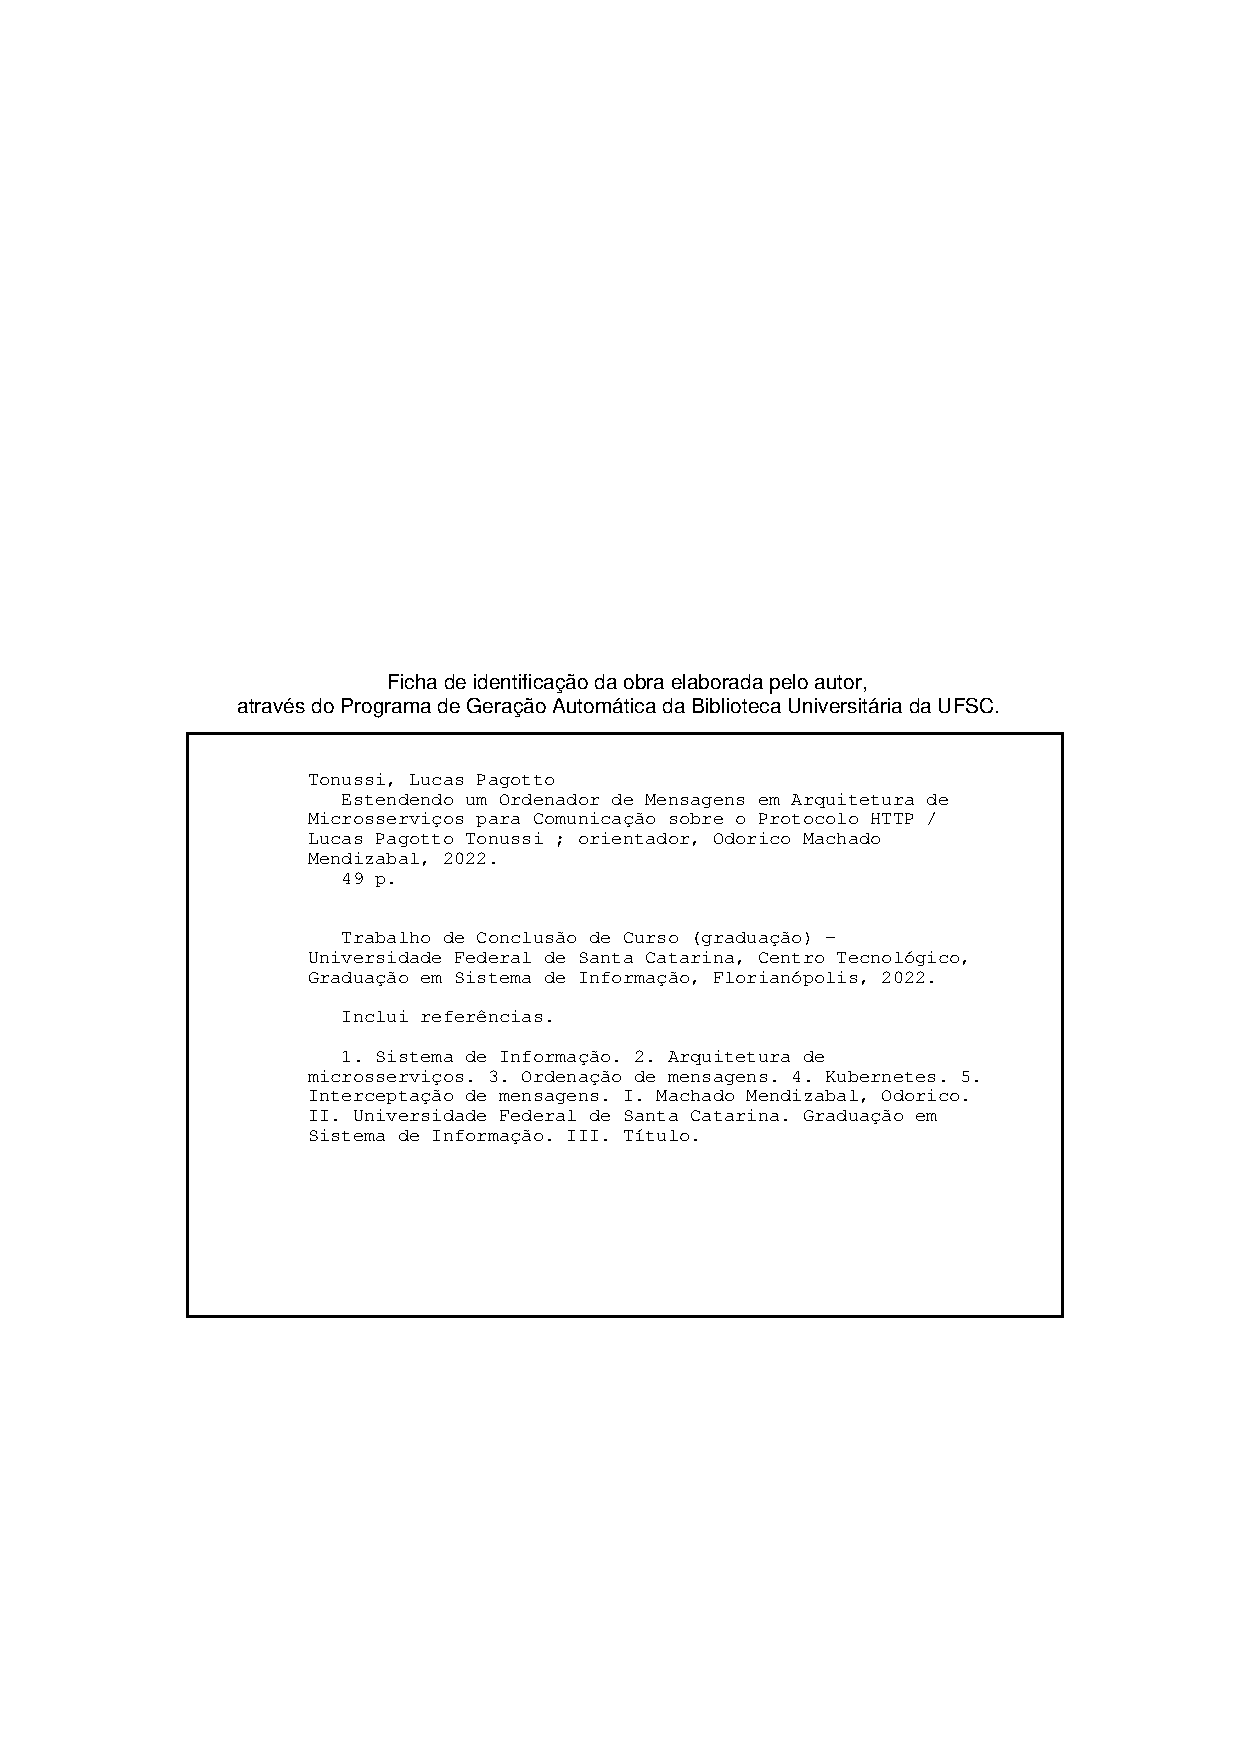
\includepdf{beforetext/Ficha_Catalografica_Preenchido.pdf}
\end{fichacatalografica}
% ---

% ---
% Inserir folha de aprovação
% ---
\begin{folhadeaprovacao}
\OnehalfSpacing
\centering
\imprimirautor\\%
\vspace*{10pt}		
\textbf{\imprimirtitulo}%
\ifnotempty{\imprimirsubtitulo}{:~\imprimirsubtitulo}\\%
% \vspace*{31.5pt}%3\baselineskip
\vspace*{\baselineskip}
%\begin{minipage}{\textwidth}
O presente trabalho em nível de \imprimirnivel~foi avaliado e aprovado por banca examinadora composta pelos seguintes membros:\\
%\end{minipage}%
\vspace*{\baselineskip}
Prof.(a) Luciana de Oliveira Rech, Dr(a).\\
Universidade Federal de Santa Catarina\\
\vspace*{\baselineskip}
Prof.(a) Alex Sandro Roschildt Pinto, Dr(a).\\
Universidade Federal de Santa Catarina\\
\vspace*{\baselineskip}
\vspace*{2\baselineskip}
\begin{minipage}{\textwidth}
% O presente trabalho é um \textbf{rascunho de monografia} para ser entregue na disciplina INE5631 (Projetos I)
Certificamos que esta é a \textbf{versão original e final} do trabalho de conclusão que foi julgado adequado para obtenção do título de \imprimirformacao.\\
\end{minipage}
% \vspace{-0.7cm}
\vspace*{\fill}
\assinatura{\OnehalfSpacing Coordenação do Programa de Pós-Graduação}
\vspace*{\fill}
\assinatura{\OnehalfSpacing\imprimirorientador \\ \imprimirorientadorRotulo}
% \ifnotempty{\imprimircoorientador}{
% \assinatura{\imprimircoorientador \\ \imprimircoorientadorRotulo \\
% \imprimirinstituicao~--~\imprimirinstituicaosigla}
% }
% \newpage
\vspace*{\fill}
\imprimirlocal, \imprimirano.
\end{folhadeaprovacao}
% ---

% ---
% Dedicatória
% ---
\begin{dedicatoria}
\vspace*{\fill}
\noindent
\begin{adjustwidth*}{}{5.5cm} 
\raggedleft       
Este trabalho é dedicado aos meus amigos íntimos, irmãos, colegas de classe e aos meus queridos pais.
\end{adjustwidth*}
\end{dedicatoria}
% ---

% ---
% Agradecimentos
% ---
\begin{agradecimentos}
Agradeço ao meu orientador Odorico Machado Mendizabal pela mentoria, ensinamentos, orientações e revisões do texto. Agradeço também ao Renan Tarouco da Fonseca pelas muitas ajudas e a Marina Milhomens Queiroz pela ajuda com a escrita.
\end{agradecimentos}
% ---

% ---
% Epígrafe
% ---
\begin{epigrafe}
\vspace*{\fill}
\begin{flushright}
\textit{``Thinking doesn't guarantee that we won't make mistakes. But not thinking guarantees that we will''\\
(LAMPORT L., 2013)}
\end{flushright}
\end{epigrafe}
% ---

% ---
% RESUMOS
% ---

% resumo em português
% ajusta o espaçamento dos parágrafos do resumo
\setlength{\absparsep}{18pt}
\begin{resumo}
\SingleSpacing

Recentemente, arquiteturas baseadas em microsserviços ganharam popularidade, em parte por causa do modelo de programação modular, acoplamento mínimo entre as partes e o suporte de plataformas de orquestração de contêineres. Ordenação de mensagens é uma estratégia que garante que todas as réplicas evoluam igualmente, aumentando-se os níveis de disponibilidade de serviços. Visando aplicações que usufruem de interfaces \gls{HTTP} para operar, este trabalho propõe uma implementação de interface de comunicação, sobre o protocolo HTTP e para um ordenador de mensagens. Sabe-se que orquestradores de contêineres oferecem replicação de forma automática, porém o serviço oferecido por orquestradores garante replicação de aplicações \textit{stateless}. O objetivo é continuar desenvolvendo um ordenador de mensagens transparente ao usuário, para isto este trabalho estende uma pesquisa iniciada pelo grupo, que propõe o Hermes, um interceptador de mensagens como serviço que usufrui de mecanismos de orquestração de contêineres para prover replicação e tolerância a falhas. O desenvolvimento do serviço de ordenação de mensagens contou com a implementação da interface que promove a comunicação no Hermes. A implementação possibilita que o Hermes possa tratar mensagens \gls{HTTP}. Ao final houve investigação de desempenho da implementação em casos específicos de vazão e latência. Os experimentos incluíram duas aplicações para avaliação de desempenho: uma aplicação de \textit{log} que recebe requisições HTTP e salva, em arquivo de disco e uma aplicação geradora de carga que envia requisições HTTP, podendo ser configurada por parâmetros. A investigação demonstrou que as latências capturadas nos geradores de carga apresentaram valores maiores para o sistema replicado quando comparado com o caso não-replicado, isto era esperado. O cenário de carga de 100\% POST, os experimentos se mostraram mais promissores. O caso onde existe 100\% de cargas GET os experimentos se mostraram melhores que no caso híbrido de 50\% GET e 50\% POST, por causa que existe 50\% de chance de múltiplos processos inserirem mais linhas no arquivo de \textit{log}. Finalmente, as comparações entre os cenários replicados e não-replicado mostraram que o ordenador de mensages prove tolerância a falhas e replicação ativa de aplicações \textit{stateful} baseadas em HTTP.

\textbf{Palavras-chave}: Protocolo de consenso. Proxy. Interceptação de Mensagens. Orquestração de contêineres. Ordenação total. Arquitetura de microsserviços. Kubernetes. Docker.
\end{resumo}


% resumo em inglês
\begin{resumo}[Abstract]
\SingleSpacing
\begin{otherlanguage*}{english}
Recently, architectures based on micro-services gained popularity, in part because of the modular programming model, minimum coupling between parts of the system and support on container orchestration platforms, also offering automatic resources management. Message ordering is a strategy that guarantees that all replicas of a distributed system will evolve equally, raising the levels of availability of services and fault tolerance. Aiming applications that use \gls{HTTP} to operate, this work proposes a implementation of a interface of communication over the \gls{HTTP} protocol and for a message ordering system. It's known that container orchestrators offers replication automatically, although that replication works, adequately, for stateless applications. This proposal aims to cover cases where the server being replicated is stateful. The objective is to continue the development of a transparent ordering system, for that the present work extends a work previously proposed by the research group, a work called Hermes, which is a service that intercepts messages and take advantage of a container orchestration system. The improvement of that message orderer service counted on a new implementation of the interface that covers communication, the implementation enables the message orderer system to handle \gls{HTTP} requests. Afterwards, benchmarks of throughput and latency were made. The experiments included two applications: a log application that receives HTTP and saves, in a disk file, the request body and a stress generator application that sends HTTP requests, and can be configured by parameters. The experiments showed that the latencies captured on the stress generators received greater numbers when compared to the non-replicated case, that was expected. The scenario where there is a 100\% load of POST requests, the experiment showed a more promising scenario. The case where there is a 100\% load of GET requests, the experiment showed better results than the 50\% GET 50\% POST mixture, because there is a 50\% chance of multiple processes inserting more lines into the file. Finally the comparisons between the replicated and non-replicated scenarios showed that the Hermes is able to tolerate failures and replicate HTTP based stateful applications.

Keywords: Consensus protocol. Proxy. Message intercepting. Container orchestration. Total ordering. Micro-services architectures. Kubernetes. Docker.

\end{otherlanguage*}
\end{resumo}

%% resumo em francês 
%\begin{resumo}[Résumé]
% \begin{otherlanguage*}{french}
%    Il s'agit d'un résumé en français.
% 
%   \textbf{Mots-clés}: latex. abntex. publication de textes.
% \end{otherlanguage*}
%\end{resumo}
%
%% resumo em espanhol
%\begin{resumo}[Resumen]
% \begin{otherlanguage*}{spanish}
%   Este es el resumen en español.
%  
%   \textbf{Palabras clave}: latex. abntex. publicación de textos.
% \end{otherlanguage*}
%\end{resumo}
%% ---

{%hidelinks
\hypersetup{hidelinks}
% ---
% inserir lista de ilustrações
% ---
\pdfbookmark[0]{\listfigurename}{lof}
\listoffigures*
\cleardoublepage
% ---

% ---
% inserir lista de quadros
% ---
% \pdfbookmark[0]{\listofquadrosname}{loq}
% \listofquadros*
% \cleardoublepage
% ---

% ---
% inserir lista de tabelas
% ---
% \pdfbookmark[0]{\listtablename}{lot}
% \listoftables*
% \cleardoublepage
% ---
\pdfbookmark[0]{\listalgorithmcfname}{lof}
\listofalgorithms
\cleardoublepage
% ---
% inserir lista de abreviaturas e siglas (devem ser declarados no preambulo)
% ---

\imprimirlistadesiglas
% ---

% ---
% inserir lista de símbolos (devem ser declarados no preambulo)
% ---
% 	\imprimirlistadesimbolos
% ---

% ---
% inserir o sumario
% ---
\pdfbookmark[0]{\contentsname}{toc}
\tableofcontents*
\cleardoublepage
}%hidelinks
% ---



